\documentclass[11pt,a4paper]{article}
\usepackage[T1]{fontenc}
\usepackage{lmodern}
\usepackage[utf8]{inputenc}
\usepackage[polish]{babel}
\usepackage{amsmath,amssymb,graphicx,xcolor,hyperref,float}
\usepackage[margin=2.35cm]{geometry}
\setlength{\emergencystretch}{1em}
\newcommand{\lang}[1]{\textcolor{blue}{#1}}
\newcommand{\substantive}[1]{\textcolor{red}{#1}}
\newcommand{\remove}[1]{\textcolor{green!50!black}{#1}}
\title{Audyt i uzupełnienie modelu kosmologicznego\\
\large do artykułu \emph{Local Maxwell symmetry and gravity}}
\author{Mira Voss i Jan Księżyc\\
\small Fikcyjny Uniwersytet Nowej Atlantydy}
\date{\today}
\begin{document}
\maketitle
\noindent\textbf{Status opracowania.} To dydaktyczny aneks do
artykułu R. Durki i J. Kowalskiego-Glikmana,
\href{https://arxiv.org/abs/1110.6812}{arXiv:1110.6812} (2011).
Nazwiska na stronie tytułowej są fikcyjnymi autorami \emph{tego aneksu},
a nie autorami oryginalnej publikacji. Wersja źródłowa
\texttt{arXiv/src/1110.6812} nie była dostępna w środowisku pracy,
dlatego poniższy dokument nie jest przerobioną pełną wersją artykułu.

\section{Legenda kolorów i audyt językowy}
\noindent\lang{Niebieski} oznacza proponowaną poprawkę językową,
\substantive{czerwony} uzupełnienie merytoryczne, a
\remove{zielony} fragment proponowany do usunięcia.
Przykłady odnoszą się do wersji HTML artykułu i nie stanowią
pełnego przeglądu wszystkich zdań:
\begin{itemize}
  \item Sekcja II: \emph{to built the action} $\to$
    \lang{\emph{to build the action}}.
  \item Sekcja II: \emph{much reacher} $\to$
    \lang{\emph{much richer}}.
  \item Dodatek A: \emph{spacial translations} $\to$
    \lang{\emph{spatial translations}}.
  \item Sekcja III: \emph{in any of these perspective} $\to$
    \lang{\emph{in any of these perspectives}}.
  \item Sekcja II: \remove{\emph{Of course}} -- w tym zdaniu
    sformułowanie nie wnosi treści do argumentu.
\end{itemize}
Zaznaczenia przedstawiają \emph{propozycje redakcyjne}.
Zastosowanie ich do całego źródła wymaga pobrania oryginalnego
archiwum TeX i ponownej kontroli kontekstu każdego zdania.

\section{Równanie z promieniowaniem}
W sekcji IV oryginalnego artykułu energia pola cechowania
spełnia równanie stanu $p=\varepsilon/3$.
Z równania ciągłości $\dot\varepsilon+4H\varepsilon=0$ wynika
$\varepsilon=\varepsilon_0(a_0/a)^4$. Po podstawieniu do
równania Friedmanna i przyjęciu $y=a^2$, $h^2=\Lambda/3$,
$C=(8\pi G/3)\varepsilon_0a_0^4$, otrzymujemy
\begin{equation}
  H^2=\frac{\Lambda}{3}+\frac{C}{a^4},
  \qquad
  \dot y^2=4(h^2y^2+C).
  \label{eq:y}
\end{equation}
\substantive{Znak $C$ nie musi być dodatni w rozważanym modelu,
ponieważ energia pola o niezwartej grupie cechowania nie jest
dodatnio określona. Każda gałąź rozwiązania wymaga sprawdzenia
warunku $h^2y^2+C\geq0$ oraz $y>0$.}

\section{Rozwiązania analityczne}
Dla gałęzi rozszerzającej się, z odpowiednim przesunięciem czasu,
równanie \eqref{eq:y} daje:
\begin{align}
\Lambda=0,\ C>0:\quad&
 y(t)=2\sqrt C\,(t-t_0),\\
\Lambda>0,\ C>0:\quad&
 y(t)=\frac{\sqrt C}{h}\sinh\!\bigl(2h(t-t_0)\bigr),\\
\Lambda>0,\ C=0:\quad&
 y(t)=y_0e^{2h(t-t_0)},\\
\Lambda>0,\ C<0:\quad&
 y(t)=\frac{\sqrt{-C}}{h}\cosh\!\bigl(2h(t-t_0)\bigr).
\end{align}
Przy $\Lambda<0$ oznaczmy
$q=\sqrt{|\Lambda|/3}$. Wtedy dla $C>0$
otrzymujemy
\begin{equation}
 y(t)=\frac{\sqrt C}{q}
 \sin\!\bigl(2q(t-t_0)\bigr)
\end{equation}
na przedziale, gdzie prawa strona jest dodatnia.
\substantive{Gałąź $\cosh$ dla $\Lambda>0$ odpowiada $C<0$,
natomiast dodatniemu $C$ odpowiada $\sinh$. Podanie obu przypadków
usuwa niejednoznaczność znaku energii w zapisanym rozwiązaniu.}
To rozwiązuje jedynie \emph{zredukowane równanie Friedmanna},
nie pełny układ równań dla pól $f(t)$ i $g(t)$.

\section{Kontrola numeryczna}
Skrypt Pythona rozwiązuje numerycznie
gałąź $\dot y=2\sqrt{h^2y^2+C}$ metodą Rungego--Kutty
czwartego rzędu dla $h=1$, $C=1$, $y(0)=1$.
Porównuje wynik z funkcją analityczną
$y(t)=\sinh(2t+\operatorname{arsinh}1)$.
Wykres pokazuje obie krzywe i bezwzględny błąd.
\par\noindent\substantive{Sprawdzenie zbieżności przez zmniejszenie kroku
jest konieczne przed interpretacją fizyczną; dopasowanie samej
krzywej nie dowodzi poprawności pełnego modelu pól cechowania.}\par
\begin{figure}[H]
  \centering
  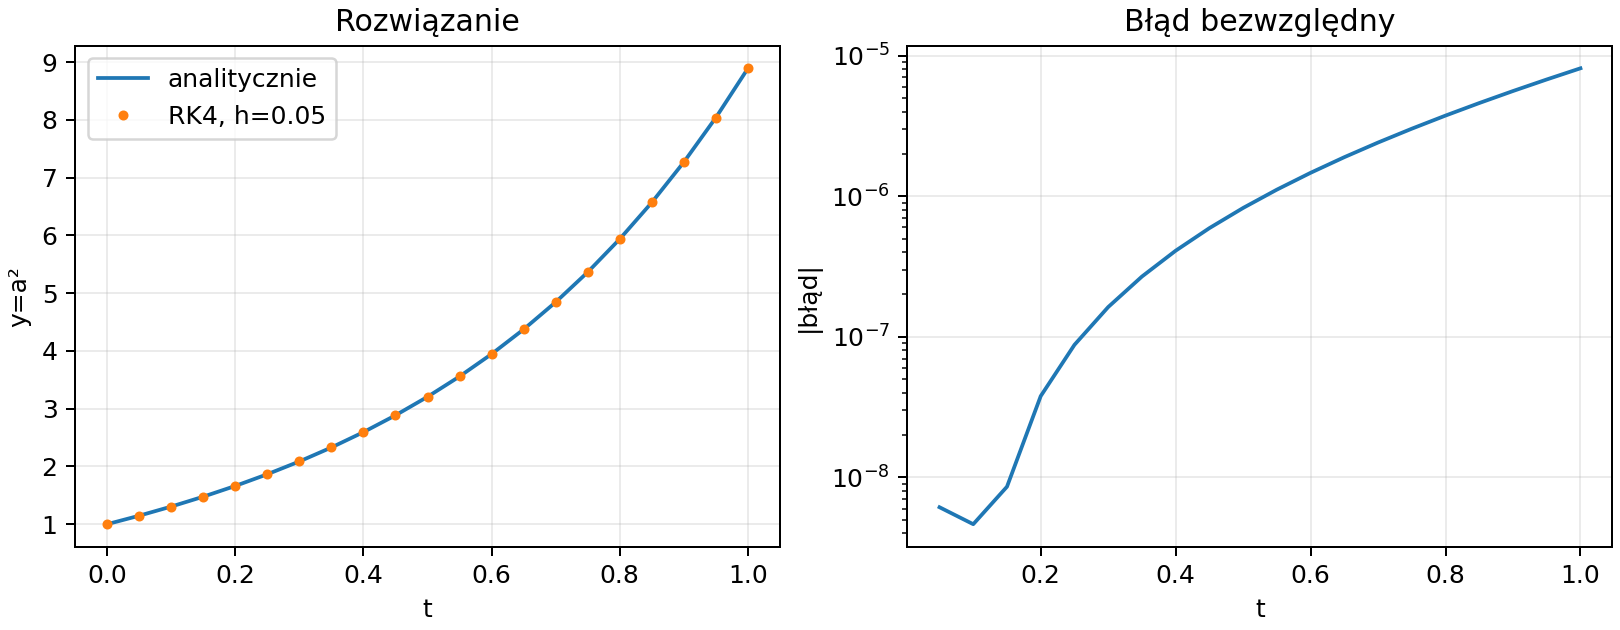
\includegraphics[width=.88\linewidth]{analiza_numeryczna.png}
  \caption{Kontrola numeryczna dodatniej gałęzi energii.
  Wielkości są bezwymiarowe.}
\end{figure}

\section{Wniosek i otwarty problem}
Redukcja kosmologiczna daje jawne rodziny funkcji $a(t)=\sqrt{y(t)}$,
ale nie ustala, które wartości $C$ są osiągalne przez rzeczywiste
rozwiązania równań pól $f$ i $g$. Dalsze badanie powinno zadać
warunki początkowe spełniające więzy, integrować połączony układ
Einsteina i równań pola oraz kontrolować więzy podczas całego przebiegu.
\end{document}
